\chapter{Data and Task Abstraction}

SynVisio was developed over multiple iterations as the necessary data and requirements were refined through continuous consultation with our genome research collaborators. To understand the design choices for visual encoding and interaction that we adopted in developing SynVisio, we need to first elaborate on the underlying data and task abstractions. We start with the data abstraction, where we explain the different characteristics of the syntenic data and how it is computed using synteny detection tools and further processed by our system. We then explore the different visual analysis tasks that can be performed on syntenic data, and finally, we discuss additional interactive and usability requirements of SynVisio that can arise when users explore complex datasets and biological scenarios.

\section{Data}
This section starts with the description of the structure of a genome and its constituent elements and follows through with an explanation of how syntenic data is generated and represented.

\subsection{Genome Structure and Scales}
The genome of every organism is unique and can be defined as the complete set of DNA needed to build and maintain that organism. Structurally, genomes are broken down into smaller sections called chromosomes, where every chromosome is a long strand of DNA coiled up along with various proteins. Each chromosome is made up of several genes, which are the basic functional units of heredity and which code for a specific protein. Genes can then be further broken down into nucleotides which are the smallest building blocks of DNA. For analyzing genomic conservation, researchers also look at a collection of collinear genes that are called blocks. Thus the genome structure can be ordered into the following five levels from top to bottom in terms of genomic size : \textit{Genome\textrightarrow{Chromosome}\textrightarrow{Block} \textrightarrow{Gene}\textrightarrow{Nucleotide}}. However, to analyze large scale genomic conservation we only look at the first four levels. The structural data of a genome describing its constituent entities is provided in the form of a \textit{GFF(General Feature Format) File}. It contains the start and end position of every gene on a linear scale in a chromosome, the gene identifier, and the reference name of the parent chromosome in a three column tab-delimited format. A partial GFF file can be seen in Figure \ref{fig:ch_3_gff_file}.  Information on several genomes belonging to different species can be presented in the same file; each species is distinguished by the two-character key present in the reference name of the chromosome. The data in the GFF file is processed by SynVisio to get the genomic size (number of nucleotides) of the different genomes and their constituent chromosomes along with the size and position of all the genes within these chromosomes. This data gives us a precise structural map of every genome and its different sub-elements and so can be used to visualize a genome over multiple scales and levels.

\begin{figure}
  \centering
  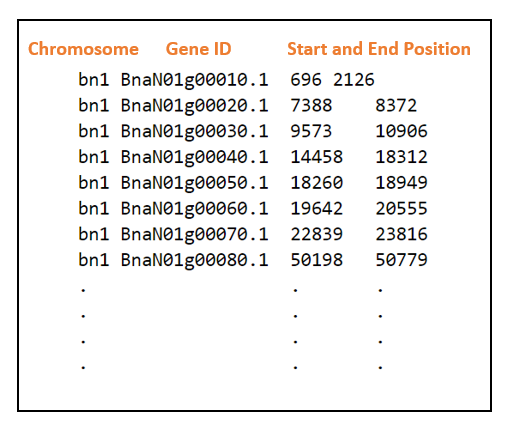
\includegraphics[width=.55\linewidth]{images/ch_3_gff_file.PNG}
  \captionof{figure}{Partial GFF file describing structure of a genome.}
  \label{fig:ch_3_gff_file}
\end{figure}


\begin{figure}
  \centering
  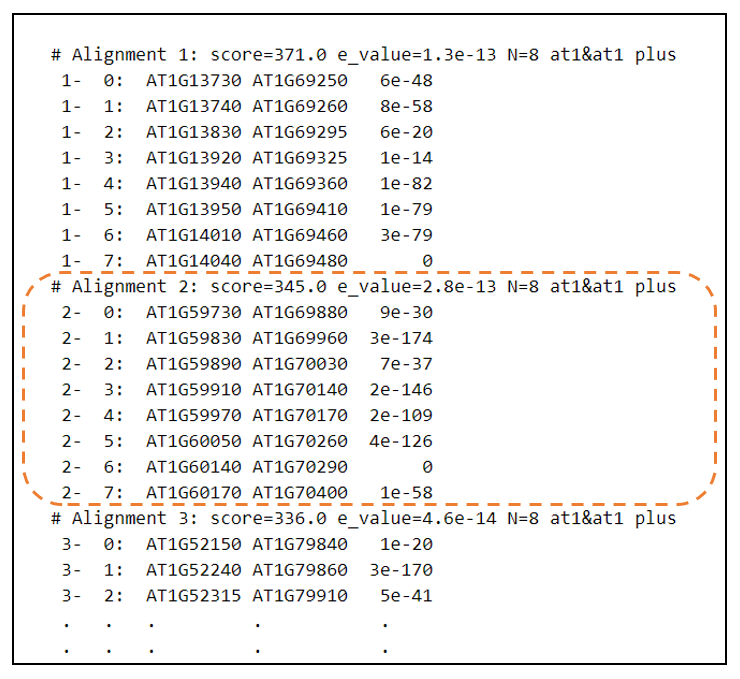
\includegraphics[width=.675\linewidth]{images/ch_3_coll_file.PNG}
  \captionof{figure}{Partial collinearity file with a single block highlighted.}
  \label{fig:ch_3_coll_file}
\end{figure}



\subsection{Conservation Data}
At the smallest level, conservation between two genes can be inferred by looking at sequence homology, which is the similarity between nucleotide sequences. Larger genomic conservation events can be studied by looking at blocks of such homologous genes and grouping them together based on their chromosomal positions to identify collinearity. To arrive at this data, we first identify all the homologous genes between two genomes using a local alignment tool such as BLAST (Basic Local Alignment Search Tool)\cite{blasttool}. Different synteny detection tools then construct collinear blocks of these homologous genes by either clustering neighbour matching gene pairs (ADHoRe, OrthoCluster) \cite{proost2011adhore,zeng2008orthocluster} or by constructing chains around an anchor gene (MCScanX)\cite{wang2012mcscanx}. These collinear blocks are referred to as syntenic blocks, and are the primary source of data for SynVisio and are provided as a collinearity file. A partial sample of a collinearity file can be seen in Figure \ref{fig:ch_3_coll_file}. Every block of collinear genes has a corresponding similarity score indicating the quality of match; an expect value (\textit{E-value}) indicating the probability that the match may have been due to chance; the count of genes; the names of the source and target chromosomes that the block of genes belong to; and the orientation of the block(forward or reverse). Finally, every block of data also consists of a list of the homologous gene pairs in that block and their statistical significance (\textit{E-value}). This data, combined with the information about the structure of the genome can be used to associate every region of a genome with its homologous regions in the other genome or within itself depending on the type of synteny under investigation.


\subsection{Auxiliary Track Data}
Since genomic data is represented as a collection of linear sequences, additional information can be provided in the form of tracks parallel to the original gene sequence structure. These tracks can contain information about genomic features such as gene density, copy number variations (CNVs), and single-nucleotide polymorphisms (SNPs). The data is provided to SynVisio in a BedGraph file format consisting of four tab-delimited values: chromosome identifier, chromosomal start position, chromosomal end position, and a data value. This information can be hierarchically grouped at the block or chromosome levels in the same way as genomic sequences and can be used to annotate the corresponding sequence structure. 

\begin{figure}
  \centering
  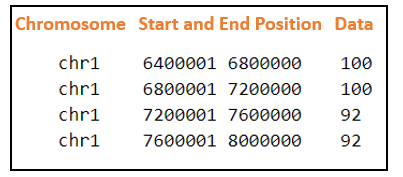
\includegraphics[width=.45\linewidth]{images/ch_3_track_file.PNG}
  \captionof{figure}{Sample track file.}
  \label{fig:ch_3_track_file}
\end{figure}

\section{Tasks}

In this section, we look at the different questions researchers have when analyzing genomic conservation. We then collate all the design requirements into a series of analysis tasks and group them based on the conservation relationship they address. Finally, we elaborate on additional interactive requirements that improve the usability of the system and assist users in performing complex analysis tasks.

\subsection{Requirement Gathering Phase}
To formulate our design requirements, we met with three groups of researchers working in different fields of biological research. The meetings were conducted over several iterations to refine our initial requirements. The sessions broadly revolved around understanding the basic tasks researchers perform when analyzing genomic conservation and looking at the shortcomings of the existing synteny analysis tools on the market. Although all three groups were primarily interested in analyzing synteny, their individual use cases varied, providing us with a diverse set of user scenarios.

Our first research group was involved in researching genomic conservation in the \textit{brassica} genus as it offers an ideal model to study polyploid evolution, which is responsible for genetic variations that are advantageous from an evolutionary perspective\cite{madlung2013polyploidy,liu2014brassica}. In particular they were interested in understanding genomic conservation within an allotetraploid species \textit{Brassica napus}(AACC), an important oilseed crop, and also in comparing it to the closely related diploid species \textit{Brassica rapa}(AA) and \textit{Brassica oleracea}(CC) that belong together in the classical triangle of U\cite{nagaharu1935genome}. The requirements from this research group were focused around having access to a system that could let them visualize the conserved relationship between the different diploid species and also within the chromosomes of a single allotetraploid (i.e. self-synteny). 

The second research team was interested in looking at genomic conservation between \textit{Lens culinaris} and \textit{Cicer arietinum} to improve various agronomic traits, as these are both widely grown legume crops. The requirements here were largely focused on cross synteny rather than self synteny. A unique trait of this particular dataset is that while \textit{C. arietinum} has a genome size of 740 Mbp, \textit{L. culinaris} has a genome size of 4 Gbp. This vast difference in the sizes of the two genomes makes visualizing synteny at the whole genome level extremely difficult and researchers must hence rely on comparing individual chromosomes of \textit{L. culinaris} one at a time or rely on a visualization that can have variable scales between the source and the target genomes.


The final research group works on sequencing wheat, and the researchers in this group were interested in understanding the genomic conservation between the three subgenomes of the hexaploid bread wheat genome. Researchers from this team wanted a system that could visualize synteny between three different genomes instead of a single source and target, while taking into consideration the extremely large size of the wheat genome. They were also interested in adopting a novel network-based visualization called a Hive Chart\cite{krzywinski2011hive}, which maps nodes onto radially distributed linear axes, for exploring multi-way genomic conservation.

\subsection{Tasks}
Broadly the requirements gathered from our research collaborators can be grouped into primary visual tasks for observing conservation and interactive system tasks for exploring complex datasets and biological scenarios. Further based on the underlying data, the primary visual tasks can be ordered into three basic groups according to the genomic scale at which they operate.

\subsubsection{Primary Visual Tasks}

\smallskip
\noindent
\textbf{Genome Level}
\smallskip
\begin{enumerate}
\item [$Q_1$.] What is the level of conservation that exists between two or more sets of genomes?
\item [$Q_2$.] How does the density of conservation change across the genomes, and are there any gaps?
\item [$Q_3$.] How does the ordering of chromosomes based on conservation change between a given set of genomes or within a single genome? (possibility of detecting whole-genome duplication or genome reversal )
\item [$Q_4$.] If unmarked scaffolds exist, which regions of the target genome do they share similarity with?
\item[$Q_5$] Which chromosomes are sparsely or entirely unaligned, and how does the level of conservation change when these are ignored ?
\end{enumerate}

\smallskip
\noindent
\textbf{Chromosome Level}
\smallskip
\begin{enumerate}
\item [$Q_6$.]What is the level of conservation between a specific subset of chromosomes?
\item [$Q_7$.] What is the level of conservation between a single chromosome and an entire target genome or several other chromosomes (detecting unaligned regions within a chromosome)?
\item [$Q_8$.] 
How large are the collinear blocks relative to neighbouring chromosomes?
\item [$Q_9$.]What is the orientation of collinear blocks between two given chromosomes? (regular or inverted)
\end{enumerate}

\smallskip
\noindent
\textbf{Block Level}
\smallskip
\begin{enumerate}
\item [$Q_{10}$.]What is the level of conservation between the set of genes in a collinear block?
\item [$Q_{11}$.] What are the different genes contained in a block?
\item [$Q_{12}$.] What is the size of a gene relative to the size of the collinear block?
\item [$Q_{13}$.] Are there large gaps between genes in collinear blocks?
\item [$Q_{14}$.] Answer $Q_{10}$-$Q_{13}$ when a collinear block is reversed?
\end{enumerate}

There are also several other analysis tasks that researchers perform that go beyond the block level and down to the nucleotide level. However, these tasks are beyond the scope of this project and there are several other systems specifically designed to investigate collinearity at the nucleotide level, such as JBrowse \cite{skinner2009jbrowse}.

\subsubsection{Interactive System Requirements}
 \begin{enumerate}
\item [$R_1$.] \textbf{Dynamic refinement of visualizations}. Synteny analysis focuses on identifying conserved regions in specific parts of the genome with the ability to focus on distant or close matches from an evolutionary perspective. Researchers need to be able to filter the generated visualizations in real time based on features of the conserved region such as the level of match and its chromosomal position. 

\item [$R_2$.] \textbf{Multiple perspectives on the dataset}. Researchers who undertake complex analysis tasks require multiple coordinated views that show different visual representations, each focusing on a particular primary feature of the dataset such as the orientation (dot plot) or the location (parallel plot). Researchers integrate the different perspectives in different ways as they carry out their tasks.

\item [$R_3$.] \textbf{Dynamic visualizations of multi-scale data}. Genetic conservation is often explored at several levels (genome, chromosome, or gene block), and the focus of analysis can be different at every genomic scale. Visualization systems should therefore allow users to switch scale quickly and easily, and should provide capabilities and interactions that adapt based on the scale of the investigation.

\item [$R_4$.] \textbf{Augmenting visualizations with secondary data}. Insights in synteny analysis can be gained by looking at conservation in the context of gene density or the positions of genetic anomalies (single nucleotide polymorphisms). Therefore, systems should offer researchers the ability to add layers of visual information onto the basic visualizations, using the main representation as a reference frame.

\item [$R_5$.] \textbf{Visualizations of multiple genomes}. Multi-way visualizations can let researcher trace conservation across several genomes, thus offering a novel way to visualize synteny combined with phylogeny (i.e., the evolutionary relationship between two species).

\item [$R_6$.] \textbf{Navigation and revisitation support}. Synteny analysis is often used in the hypothesis-generation stage of research, requiring that genome scientists explore several scenarios through the analysis tool. This can be problematic when genomes are large (e.g., the wheat genome is 17 Gbases -- six times larger than the human genome), because researchers can easily lose context of their location in the genome (particularly in polyploid organisms where genes are duplicated multiple times). In addition, a complex visualization system also presents a large "parameter space" requiring that users remember the settings and navigation actions that brought them to their current viewpoint. Analysis tools therefore need to support navigation and record provenance in order to enable communication between collaborators and to enable revisitation of potentially-interesting locations during exploration.

\end{enumerate}
